\chapter{Pré-requis et installation}
\label{chap-setup}

\renewcommand{\headrulewidth}{0.3pt}
\fancyhead[LE]{\thepage}
\fancyhead[RE]{\nouppercase{\textbf{\leftmark}}}
\fancyhead[RO]{\thepage}
\fancyhead[LO]{\nouppercase{\textbf{\rightmark}}}
\fancyfoot[L,C,R]{}

\setlength{\parindent}{0.35cm}

\minitoc
\newpage

% ================================================================

Le plug-in \cwv~a été conçu pour fonctionner sous le système d'information géographique (SIG) QGIS. Il a initialement été développé sous QGIS 3.28\footnote{Disponible à l'adresse : \href{https://www.qgis.org/fr/site/forusers/download.html}{https://www.qgis.org/fr/site/forusers/download.html}}, et est actuellement utilisé sous sa version 3.36. Son bon fonctionnement n'est pas garanti pour une utilisation sous une version ultérieure.

\cwv~s'appuie sur un backend scientifique, \script{HydrologicalTwinAlphaSeries} (HTAS), embarqué dans le dépôt comme sous-module \gitlab~sous \script{external/HydrologicalTwinAlphaSeries}. Ce sous-module doit être renseigné pour que le plug-in puisse fonctionner, quelle que soit l'option d'installation retenue.

Deux options d'installation sont disponibles :
\begin{itemize}
    \item \textbf{Option 1 --- environnement Pixi} (\cref{sec-install-pixi}) : installe QGIS et l'ensemble des dépendances à l'intérieur du dossier du projet, de manière reproductible et autonome. Recommandée pour les développeurs et pour des déploiements reproductibles.
    \item \textbf{Option 2 --- gestionnaire d'extensions QGIS via ZIP} (\cref{sec-install-user}) : l'archive de plug-in classique, installée depuis QGIS. Plus pratique pour les utilisateurs finaux, mais plus fragile pour la gestion des dépendances.
\end{itemize}

\section{Option 1 --- environnement Pixi (recommandée)} \label{sec-install-pixi}

Cette option installe QGIS et l'ensemble des dépendances à l'intérieur du dossier du projet \textit{via} \href{https://pixi.sh}{\script{pixi}}. Elle fournit un environnement reproductible et autonome dans lequel QGIS, Python et chaque dépendance sont figés.

\subsection{Installer \script{pixi} (une fois par machine)}
Voici les informations reprises de la \href{https://pixi.prefix.dev/latest/installation/#__tabbed_1_1}{page d'installation de Pixi} :

Sous macOS ou Linux :
\begin{lstlisting}[language=bash]
curl -fsSL https://pixi.sh/install.sh | sh
source $HOME/.bashrc
\end{lstlisting}

Si votre système ne dispose pas de \script{curl}, utilisez \script{wget} :
\begin{lstlisting}[language=bash]
wget -qO- https://pixi.sh/install.sh | sh
\end{lstlisting}

Sous Windows :
\begin{lstlisting}[language=bash]
powershell -ExecutionPolicy Bypass -c "irm -useb https://pixi.sh/install.ps1 | iex"
\end{lstlisting}

\subsection{Cloner le dépôt, initialiser le backend et installer l'environnement}

\begin{lstlisting}[language=bash]
mkdir $HOME/.plugins-qgis
cd $HOME/.plugins-qgis
git clone https://gitlab.com/gviz/cawaqsviz.git
cd cawaqsviz
git submodule update --init external/HydrologicalTwinAlphaSeries
pixi install
\end{lstlisting}

Depuis la racine du dépôt \script{cawaqsviz}, initialisez uniquement \script{external/HydrologicalTwinAlphaSeries}. N'utilisez pas de mise à jour récursive des sous-modules, sauf si vous avez explicitement besoin des sources de la documentation interne du backend et que vous avez accès à leurs dépôts privés.

\subsection{Lancer QGIS}

\begin{lstlisting}[language=bash]
pixi run cawaqsviz
\end{lstlisting}

La dernière étape consiste à activer le plug-in dans QGIS depuis le menu principal : \gui{Extensions} $\rightarrow$ \gui{Installer/Gérer les extensions}, puis à sélectionner \gui{Installées} dans la fenêtre de navigation qui s'ouvre (\cref{fig-CWV-activation}).

\subsection{Mettre à jour le plug-in} \label{sec-install-pixi-update}

Une fois l'installation effectuée, placez-vous dans le répertoire \script{cawaqsviz}, mettez-le éventuellement à jour vers la dernière version, puis lancez-le avec \script{pixi} :

\begin{lstlisting}[language=bash]
cd $HOME/.plugins-qgis/cawaqsviz
git pull                                                          # met a jour cawaqsviz ; peut deplacer le SHA fige du backend
git submodule sync -- external/HydrologicalTwinAlphaSeries        # rafraichit l'URL distante du backend si elle a change en amont
git submodule update --init external/HydrologicalTwinAlphaSeries  # place le backend sur le SHA fige par cawaqsviz
pixi run cawaqsviz                                                # lance QGIS depuis l'environnement pixi
\end{lstlisting}

\section{Option 2 --- gestionnaire d'extensions QGIS via ZIP} \label{sec-install-user}

L'outil de visualisation \cwv~a été développé et testé sous QGIS 3.28 et versions ultérieures. ATTENTION : ce type d'installation est plus fragile que l'Option 1 pour la gestion des dépendances. L'équipe de développement recommande l'Option 1 pour le développement à partir des sources et pour des environnements reproductibles.

\alertwarning{N'utilisez \textbf{pas} le bouton \gui{Download ZIP} de \gitlab~--- son archive casse l'installation du plug-in. Vous devez construire le ZIP vous-même à partir d'un \script{git clone} correct incluant le contenu des sous-modules, comme indiqué ci-dessous.}

\noindent Le téléchargement de l'archive \gitlab~échoue pour deux raisons :
\begin{itemize}
    \item le dossier de premier niveau porte le nom de la branche ou du tag (par ex. \script{cawaqsviz-main-abc1234/}), alors que QGIS exige qu'il soit nommé exactement \script{cawaqsviz}. L'installation directe du ZIP \gitlab~produit une erreur du type \script{No module named 'cawaqsviz-<branch>'} ;
    \item le contenu des sous-modules \gitlab~n'est pas inclus --- seulement un pointeur. Le dossier embarqué \script{external/HydrologicalTwinAlphaSeries/} sera vide et l'amorçage au premier lancement échouera avec une erreur de type « sous-module manquant ».
\end{itemize}

\subsection{Construire un ZIP d'installation propre}

Sous Linux/macOS :
\begin{lstlisting}[language=bash]
# 1. Cloner dans un emplacement temporaire avec le contenu des sous-modules
cd /tmp
git clone https://gitlab.com/gviz/cawaqsviz.git
cd cawaqsviz
git submodule update --init external/HydrologicalTwinAlphaSeries

# 2. Construire le ZIP depuis le repertoire parent, en excluant (facultatif) les artefacts propres au developpement
cd ..
zip -r cawaqsviz.zip cawaqsviz \
    -x "cawaqsviz/.git/*" \
    -x "cawaqsviz/.pixi/*" \
    -x "cawaqsviz/__pycache__/*" \
    -x "cawaqsviz/**/__pycache__/*"
\end{lstlisting}

Sous Windows (PowerShell), utilisez Git for Windows pour cloner (les mêmes commandes \script{git} que ci-dessus), puis construisez le ZIP en cliquant droit sur le dossier \script{cawaqsviz/} ($\rightarrow$ \gui{Envoyer vers} $\rightarrow$ \gui{Dossier compressé}), ou avec PowerShell :
\begin{lstlisting}[language=bash]
Compress-Archive -Path cawaqsviz -DestinationPath cawaqsviz.zip
\end{lstlisting}

Le \script{cawaqsviz.zip} obtenu porte le bon nom de dossier de premier niveau et inclut le contenu du sous-module backend.

\subsection{Installer le ZIP dans QGIS}

Dans la barre supérieure de menus de QGIS, cliquez sur \gui{Extensions} puis \gui{Installer/Gérer les extensions}. La fenêtre de gestion et d'import des extensions s'ouvre. Sélectionnez \gui{Installer depuis un ZIP} (\cref{fig-QGIS_install_from_zip}) et choisissez \script{cawaqsviz.zip}, puis cliquez sur \gui{Installer l'extension}.

\begin{figure}[H]
    \centering
    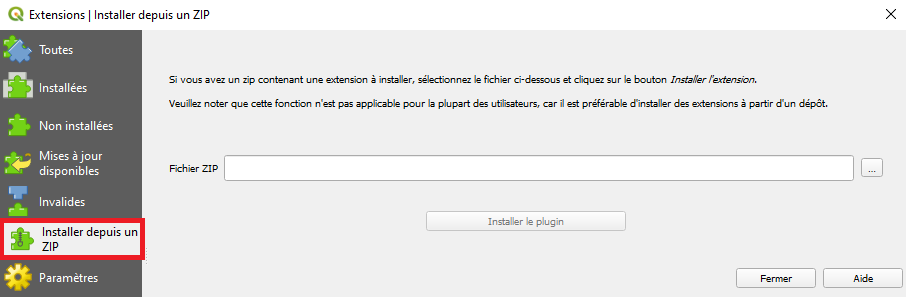
\includegraphics[width=1\linewidth]{1_installation_requirements/fig/QGIS_install_from_zip.png}
    \caption{Boîte de dialogue QGIS pour la gestion d'extensions.}
    \label{fig-QGIS_install_from_zip}
\end{figure}

Une fois le fichier \script{.zip} décompressé sous QGIS, il peut être nécessaire d'activer ce dernier dans la même fenêtre de gestion des extensions en naviguant dans le volet \gui{Installées}. L'extension \cwv~doit être cochée pour figurer dans la barre d'outils QGIS (\cref{fig-CWV-activation}).

\begin{figure}[H]
    \centering
    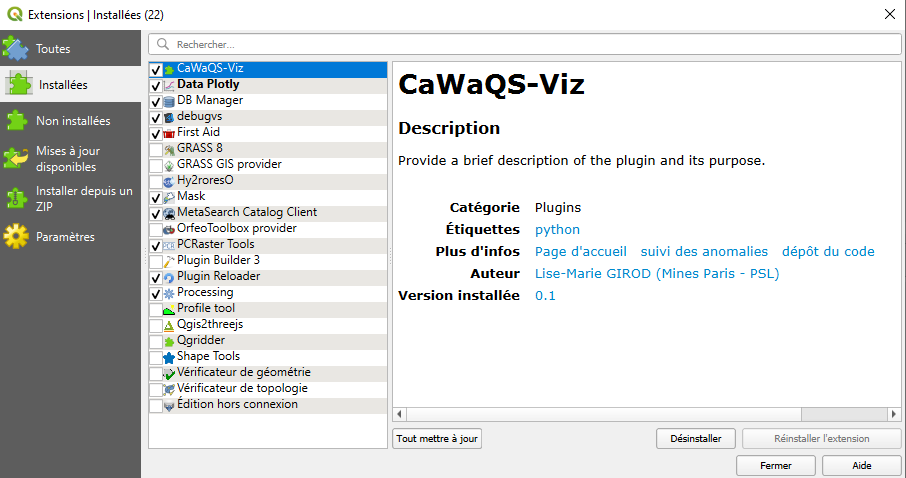
\includegraphics[width=1\linewidth]{couverture/fig/QGIS_get_plugin_in_toolbar.png}
    \caption{Activation de l'extension \cwv~dans l'application QGIS.}
    \label{fig-CWV-activation}
\end{figure}

Une fois l'application présente dans la barre d'outils de QGIS, celle-ci est prête à être lancée d'un simple clic sur l'icône 
\includegraphics[height=0.45cm]{couverture/fig/Icon_CaWaQSVIZ.png}.

\subsection{Ce qui se passe au premier lancement} \label{sec-install-bootstrap}

Au premier lancement après une installation par ZIP, le plug-in exécute automatiquement \script{pip install --user --upgrade external/HydrologicalTwinAlphaSeries} pour enregistrer le backend et résoudre ses dépendances Python. Cela nécessite une connexion internet et s'installe dans les site-packages propres à votre utilisateur (\script{\textasciitilde/.local/lib/pythonX.Y/site-packages} sous Linux, \script{\%APPDATA\%\textbackslash Python\textbackslash...} sous Windows). Les lancements suivants sont sans effet.

Sous Debian/Ubuntu et dérivés qui embarquent un Python système « externally-managed » (PEP~668), le plug-in retente automatiquement avec \script{--break-system-packages} (l'installation atterrit tout de même dans vos site-packages utilisateur, et non dans les chemins système gérés par apt).

Si l'installation échoue, la console Python de QGIS affiche la commande \script{pip} exacte que vous pouvez exécuter manuellement pour diagnostiquer.

\alertinfo{Pour utiliser toute nouvelle mise à jour du plug-in installé via ZIP, il sera nécessaire de réitérer l'intégralité de cette procédure (\cref{sec-install-user}). Avec l'Option 1, la mise à jour se fait plutôt avec \script{git pull} (\cref{sec-install-pixi-update}).}

\section{Paramètres d'installation avancés (DEV)} \label{setup-dependances}
\subsection{Installation des dépendances}
Les dépendances sont gérées automatiquement. Avec l'Option 1, \script{pixi} fige et installe QGIS, Python et chaque dépendance à l'intérieur du dossier du projet (\cref{sec-install-pixi}). Avec l'Option 2, l'amorçage au premier lancement résout le backend et ses dépendances Python (\cref{sec-install-bootstrap}). Aucune installation manuelle de dépendances n'est normalement nécessaire.

\alertinfo{Si l'amorçage au premier lancement échoue, la console Python de QGIS affiche la commande \script{pip} exacte à exécuter. En dernier recours, les dépendances peuvent tout de même être installées manuellement depuis l'interpréteur Python intégré à QGIS. Les installer depuis un autre interpréteur ne permettra pas à QGIS d'accéder aux librairies nécessaires.}

Les principales dépendances Python sont : \script{pandas}, \script{numpy}, \script{ipython}, \script{matplotlib} et \script{geopandas}. En solution de repli manuelle, ouvrez une console Python de QGIS\footnote{En cliquant sur 
\includegraphics[height=0.45cm]{1_installation_requirements/fig/interpreteur_python.png} dans l'interface QGIS.} et exécutez :

\begin{lstlisting}[language=python]
>>> import pip
>>> pip.main(['install', 'pandas', 'numpy', 'ipython', 'matplotlib', 'geopandas'])
\end{lstlisting}

\subsection{Installation pour les développeurs} \label{sec-install-expert}

À des fins de développement, et pour faciliter la mise à jour du plug-in depuis l'interface QGIS, le plug-in peut être installé directement dans le répertoire des extensions \emph{natives} de QGIS. Le dépôt \gitlab~de \cwv~peut être cloné depuis un terminal de commande, en pensant à initialiser le sous-module backend :

\begin{lstlisting}[language=bash]
$ git clone https://gitlab.com/gviz/cawaqsviz
$ cd cawaqsviz
$ git submodule update --init external/HydrologicalTwinAlphaSeries
\end{lstlisting}

Le répertoire de l'application doit être placé à l'emplacement (dossier) des applications natives de QGIS afin que toute modification du code source du plug-in puisse être prise en compte par QGIS lors de son démarrage. Le répertoire QGIS est accessible \textit{via} le chemin suivant :

\begin{lstlisting}[language=bash]
#windows
C:/Programmes/QGIS3.X.X.X/apps/qgis-ltr/python/plugins/
#linux
~/.local/share/QGIS/QGIS3/profiles/default/python/plugins/
\end{lstlisting}


La structure du code du plug-in est décrite au chapitre \ref{chap-description-src}.\\

\alertinfo{L'autocomplétion des fonctionnalités liées à la librairie qgis est disponible à condition d'utiliser l'interpréteur Python employé par QGIS. Un environnement virtuel peut être initialisé à cet effet.}

\textbf{N.B.} : Pour faciliter le développement du plug-in, les utilitaires suivants peuvent être installés depuis le gestionnaire des applications QGIS :
\begin{enumerate}
    \item \textbf{Reloader} permet de recharger le plug-in sans relancer QGIS à chaque modification de code,
    \item \textbf{FirstAid} permet une visualisation détaillée des erreurs retournées par l'interpréteur Python de QGIS ainsi que des différents objets et variables liés à l'extension.
\end{enumerate}
